\documentclass[10pt,a4paper]{article}
\usepackage[utf8]{inputenc}
\usepackage[italian]{babel}
\usepackage{amsmath}
\usepackage{amsfonts}
\usepackage{amssymb}
\usepackage{graphicx}
\usepackage[left=2cm,right=2cm,top=2cm,bottom=2cm]{geometry}
\newcommand{\rem}[1]{[\emph{#1}]}

\author{Gruppo AC \\ Federico Belliardo, Giulia Franchi, Francesco Mazzoncini}
\title{Esercitazione N.4: Amplificatore a transistor}
\begin{document}

\maketitle

\section{Scopo dell'esperienza}
L'esercitazione ha come scopo quello di realizzare un circuito amplificatore, utilizzando un transistor \textit{npn} 2N1711.

\section{Montaggio del circuito e verifica del punto di lavoro}

\begin{figure}[!htb]
  \centering
  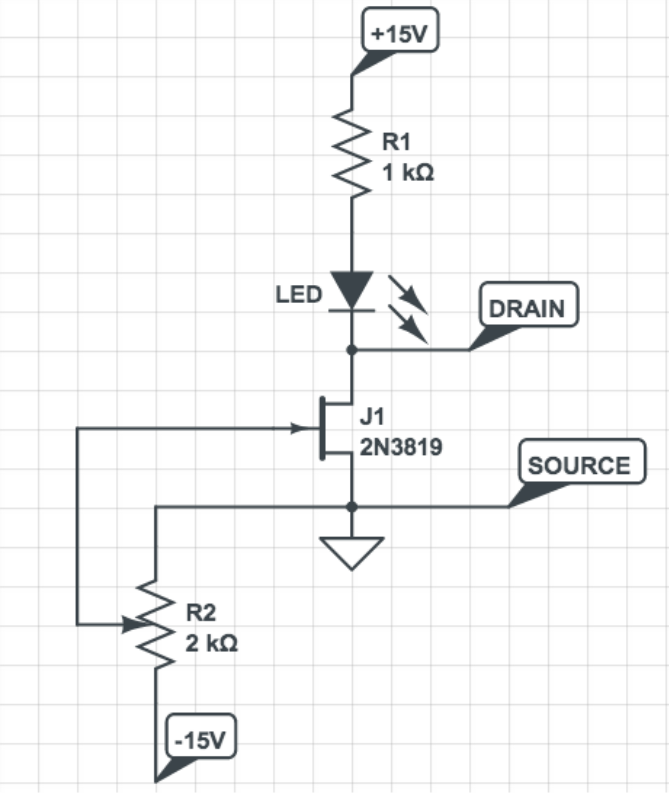
\includegraphics[scale=0.3]{circuito1.png}
\caption{Schema amplificatore a transitor.}
\label{circuito}
\end{figure}

Abbiamo montato il circuito in figura \ref{circuito} senza però inserire $R_{es}$ e $C_E$ come richiesto, con: $R_1= 179\pm1  k\Omega$, $R_2= 18.0\pm0.1  k\Omega$, $R_C= 9.95\pm 0.09  k\Omega$, $R_E= 0.987\pm 0.008 \, k\Omega$, $C_{IN}= 230\pm10  nF$ e $C_{OUT}= 99\pm4  nF$. Tutti i componenti sono stati misurati con multimetro digitale, tranne il condensatore elettrolitico di cui abbiamo assunto il valore nominale. Nei calcoli teorici seguenti supponiamo che il transistor lavori in zona attiva: $V_{BE} \simeq 0.7 \pm 0.1 \, V$.\\ 
Abbiamo inoltre definito $V_{PART}=V_{CC}\frac{R_2}{R_1+R_2}$, per determinarla abbiamo misurato la tensione in ingresso $V_{CC}= 20.2\pm0.1 V$, così la tensione ai capi del partitore risulta $V_{PART}=1.85 \pm 0.01\,V$.


\subsection{Misura del punto di lavoro}
Per la determinazione del punto di lavoro del circuito si è misurato $V_{CE}= 7.50\pm0.04 \, V$ e la caduta di potenziale ai capi della resistenza $R_C$, $V_{R_C}= 11.62\pm0.05  V$, in modo da poter determinare $I_C=\frac{V_{RC}}{I_C} = 1.17\pm0.01\,mA$.
Confrontando questi valori misurati con i valori teorici, $I_C=\frac{V_{PART}-V_{BE}}{R_E}= 1.12\pm0.01\,mA$ e $V_{CE}=V_{CC}-(R_C+R_E)I_C= 7.4\pm0.1\,V$, si vede che si ha compatibilità entro l'errore.\\
La retta di lavoro attesa è  $V_{CC}=V_{CE}+I_C(R_C+R_E)$.


\subsection{Misura delle tensioni ai terminali del transistor}
Abbiamo misurato le tensioni $V_B= 1.77\pm0.01V$, $V_E= 1.17\pm0.01V$, $V_{BE}= 0.605\pm0.004V$ e $V_C= 8.47\pm0.04V$. $V_B$ non è compatibile con il valore $V_{B\,ATT}= V_{PART}=1.85 \pm 0.01V$, probabilmente ciò si verifica poichè il partitore non è perfettamente \emph{stiff}. $V_{BE}$ rientra nell'intervallo di tensione ai capi di una giunzione a silicio polarizzata inversamente  $V_{BE} \simeq 0.7 \pm 0.1 V$. Per quanto riguarda $V_E$ e $V_C$ risultano essere compatibili entro l'incertezza con i valori attesi $V_E=I_C^Q R_E = 1.2 \pm 0.1 V$, $V_C=V_{CC}-I_C^Q R_C = 8 \pm 1 V$.


\subsection{Valutazione della corrente di base}
Ci aspetteremmo una corrente di base $I_B=\frac{I_C}{h_{FE}} = 6.9 \pm 0.4 \, \mu A$, dato che si suppone il transistor lavori in zona attiva. Dalle misure prima effettuate di $V_B$ e $V_{CC}$ ricaviamo: $I_{R1} = 98.3\pm0.8 \, \mu A$ e $I_{R2} = 103.0\pm0.8 \, \mu A$, dalle quali infine calcoliamo $I_B=I_{R1}-I_{R2}= 5\pm1 \,\mu A$. Notiamo che $I_B/I_{R1}\simeq 5\%$, quindi il partitore è ragionevolmente \emph{stiff}, anche se come visto nel paragrafo precendente questa ipotesi non è compatibile con la tensione di base $V_B$ misurata applicando la formula del partitore.
 
\section{Risposta a segnali sinusoidali di frequenza fissa}
In questa parte dell'esperienza si è utilizzato un segnale ad una frequenza fissa pari a $f= 5.00\pm0.05 \, kHz$.

\subsection{Misura del guadagno in tensione}
Abbiamo preso diverse misure di $V_{OUT}$ (a dello sfasamento di tempo rispetto all'ingresso) in funzione di $V_{IN}$ (cioè al variare di quest'ultimo) prestando attenzione ai fenomeni di clipping. Nella tabella \ref{ampiezza} seguente riportiamo le nostre misure, aggiungendo anche il calcolo del guadagno in tensione: $A_V=\frac{V_{OUT}}{V_{IN}}$ e dello sfasamento angolare rispetto a $\pi \,rad$.L'oscilloscopio è stato utilizzato in modalità AC.\\
Tutti i dati mostrati nelle tabelle e nei grafici (in tutta la relazione) riportano sia l'errore sistematico (del $3\%$) che che quello statistico (lettura del cursore dell'oscilloscopio) sommati in quadratura, in tutti i fit sono stati considerati solo gli errori statistici.

\begin{table}[!hbt]
\centering
\begin{tabular}{|c|c|c|c|c|c|}
\hline 
$V_{IN}$ [V] & $\sigma V_{IN}$ [V] & $V_{OUT}$ [V]& $\sigma V_{OUT}$ [V] & $A_V$ & $\sigma A_V$ \\ 
\hline
0.21 & 0.08 & 2.00 & 0.06 & 9.7 & 0.4\\
0.29 & 0.09 & 2.86 & 0.09 & 9.7 & 0.4\\
0.5 & 0.1 & 5.0 & 0.2 & 9.8 & 0.4\\
0.6 & 0.1 & 6.0 & 0.2 & 9.6 & 0.4\\
0.7 & 0.1 & 6.9 & 0.3 & 9.7 & 0.4\\
0.8 & 0.2 & 7.7 & 0.5 & 9.6 & 0.4\\
0.9 & 0.2 & 8.7 & 0.5 & 9.7 & 0.4\\
1.0 & 0.2 & 9.9 & 0.3 & 9.6 & 0.4\\
1.1 & 0.2 & 10.6 & 0.3 & 9.5 & 0.4\\
1.2 & 0.2 & 11.5 & 0.3 & 9.5 & 0.4\\
1.3 & 0.2 & 12.6 & 0.4 & 9.7 & 0.4\\
\hline
\end{tabular}
\caption{Misure di tensione, guadagno e fase.} \label{ampiezza}
\end{table}


Si può vedere come il segnale in uscita sia sfasato di $\pi \, rad$ come atteso dai calcoli teorici. Tutte le misure dello sfasamento sono compatibili con zero entro l'errore sperimentale. Tuttavia si può osservare una fase sistematicamente maggiore di $\pi \, rad$ probabilmente a causa dell'impedenza dei condensatori in ingresso e uscita. Il valore medio dell'attenuzione (con errore propagato in maniera statistica sulla media di tutte le misure) è: $A = 9.65 \pm 0.2$.

La tensione misurata a cui inizia il \emph{clipping} inferiore è circa $V_{inf} = 1.4 \,V$, mentre il clipping superiore inizia circa a $V_{sup} = 2.2 \, V$. Per referenza si gurdi la figura \ref{clipping}.\\
Questo è dovuto al fatto che il punto di quiescenza scelto è più vicino alla zona di saturazione che alla zona di interdizione. Il clipping inferiore corrisponde alla zona di saturazione, perchè significa che $V_{IN}$ ha il valore massimo e quindi la corrente di base è tale da mandare il transistor in saturazione.\\
Quando si ha clipping superiore la $V_{IN}$ è al minimo valore dunque non ho polarizzazione della base e sono in interdizione.
Entrambi i fenomeni accennati sono effetti non lineari del transistor, cioè deviazioni dal comportamento ideale in cui vengono mandati segnale armonici in segnali armonici.\\

\begin{figure}[!htb]
  \centering
  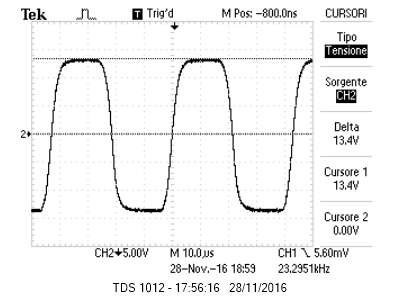
\includegraphics[scale=1.0]{clipping.png}
\caption{Il segnale a cui si vede il \emph{clipping} è $V_{OUT}$, l'altro (sfasato di $\pi \, rad$) è il segnale $V_{IN}$.}
\label{clipping}
\end{figure}

\subsection{Impedenza di ingresso del circuito}
Come impedenza in ingresso del circuito ci aspettiamo $R_{IN}=R_1//R_2//(h_{ie}+h_{fe}R_E) = 15.3\pm0.1 k \Omega$.
Abbiamo misurato la tensione in uscita del circuito in Fig \ref{circuito}: $V_{OUT,1} = (6.44\pm0.02) \, V$, e successivamente abbiamo inserito una resistenza, $R_S= (18.1\pm0.1) \, k\Omega$, fra il generatore e $C_{IN}$, misurando poi $V_{OUT,2}= (2.94 \pm 0.02) \, V$. Si misura il valore della tensione in ingresso $V_{IN} = (668 \pm 2) \, mV$, che rimane costante durate le due misure. Utilizzando la formula $\frac{R_S}{R_{IN}}=\frac{V_{OUT,1}}{V_{OUT,2}}-1$ ci è stato possibile ricavare il valore dell'impedenza in ingresso, $R_{IN}= 15.2\pm0.2\, k\Omega$. 
Per il calcolo della resistenza di ingresso teorica la resistenza dinamica della giunzione è stata stimata dalla misure prese assumendo il coefficiente $h_{fe} = 170\pm10$ determinato nella scorsa esperienza. Si ottiene un accordo ottimo della misura e della stima teorica

\subsection{Impedenza di uscita del circuito}
Come impedenza di uscita del circuito ci aspettiamo $R_{OUT}= R_C = 9.95\pm0.09\, k\Omega$. Come in precedenza abbiamo effettuato due misure di tensione: la prima con il circuito di partenza, che ha fornito:  $V_{OUT,1}= (6.40\pm0.02) \, V$ mentre la seconda è stata presa dopo aver inserito tra l'uscita e la massa una resistenza di carico $R_L = (10.05 \pm 0.08) \, k\Omega$, $V_{OUT,2}= (3.62\pm0.02)\,V$. La tensione in ingresso è: $V_{IN} = 664 \pm 2 \,mV$ sempre costante durante le misure (è stato verificato!). Grazie alla formula $\frac{R_{OUT}}{R_{L}}=\frac{V_{OUT,1}}{V_{OUT,2}}-1$ abbiamo ottenuto $R_{OUT}= (9.5\pm0.8)\, k\Omega$, in accordo entro l'errore con al resistenza teorica $R_C$.


\section{Risposta in frequenza}
Abbiamo misurato la risposta in frequenza del circuito variando la frequenza da $10Hz$ a $1MHz$, con una tensione in ingresso $V_{IN,pp}= 1.00 \pm 0.01\, V$. Quest'ultima è stata controllata più volte durante l'esperienza per far si che rimanesse costante durante la presa dati. Nella tabella sottostante sono riportate le misure effettuate. L'errore sulle frequenze (determinate grazie al frequenzimetro interno dell'oscilloscopio) è stato assunto essere l'$1\%$, poichè questo è anche l'errore che commettiamo misurando la frequenza indirettamente cioè tramite una lettura del cursore dei tempi.\\

Le misure sono state poi riportate in un diagramma di Bode. Abbiamo eseguito un fit a tre rette del diagramma per determinare la frequenze di taglio superiori e inferiori. Di seguito sono riportate i parametri delle tre rette e le frequenze determinate. L'incertezza sulle intersezioni (ottenute con la formula: $x = \frac{a_1-a_2}{b_2-b_1}$) è stata propagata grazie alla matrice di covarianza ottenuta nel fit. 

\begin{table}[!htb]\centering
\begin{tabular}{|c|c|c|c|}
\hline
$V_{OUT} (V)$ & $\sigma V_{OUT} (V)$ & $f(kHz)$ & $\sigma f (kHz)$\\
\hline
2.02 & 0.06 & 0.0103 & 0.0001\\
3.4 & 0.1 & 0.0178 & 0.0002\\
4.7 & 0.1 & 0.0262 & 0.0003\\
5.8 & 0.2 & 0.0341 & 0.0003\\
6.3 & 0.2 & 0.0408 & 0.0004\\
8.4 & 0.3 & 0.0803 & 0.0008\\
8.9 & 0.3 & 0.118 & 0.001\\
9.5 & 0.3 & 0.432 & 0.004\\
9.5 & 0.3 & 0.752 & 0.008\\
9.5 & 0.3 & 1.03 & 0.01\\
9.6 & 0.3 & 5.13 & 0.05\\
9.5 & 0.3 & 9.7 & 0.1\\
9.1 & 0.3 & 31.5 & 0.3\\
7.8 & 0.2 & 66.5 & 0.7\\
5.2 & 0.2 & 141 & 1\\
3.6 & 0.1 & 223 & 2\\
2.76 & 0.09 & 303 & 3\\
2.18 & 0.08 & 380 & 4\\
1.70 & 0.05 & 505 & 5\\
1.03 & 0.03 & 796 & 8\\
0.85 & 0.03 & 1000 & 10\\
\hline
\end{tabular}
\caption{Tensioni in uscita in funzione della frequenza.}
\label{bode}
\end{table}

Si osserva che nell'intervallo tra $100\,Hz$ e $100\,kHz$ il guadagno rimane circa costante, questo giustifica la scelta tra $1 \, kHz$ e $10 \, kHz$ della frequenza per eseguire le misure della prima parte.

Il grafico \ref{tutteBode} riporta tutte le misure effettuate, con la frequenza in scala logaritmica.

\begin{figure}[!htb]
\centering
  \includegraphics[scale = 0.4]{bodeTutti.png}
\caption{Diagramma di Bode completo.}
\label{tutteBode}
\end{figure}


Abbiamo eseguito tre fit numerici con la funzione \emph{curvefit} della libreria \emph{pylab} con l'opzione \emph{$absolute\,sigma = "true"$}, poichè abbiamo considerando gli errori come statistici, in quanto abbiamo preso soltanto l'errore sul cursore (l'errore di calibrazione è da ritenersi di tipo sistematico ed è quindi stato consderato soltanto nel grafico in figira \ref{tutteBode}, non nei fit). Questo porta alla sottostima degli errori dunque alla sovrastima del $\chi^2$. Riportiamo i grafici in figure \ref{salita}, \ref{orizz}, \ref{discesa} e i parametri fittati con la relativa matrice di covarianza.

\begin{itemize}
\item \textbf{Fit parte di salita del diagramma di Bode.}

\begin{figure}[!htb]
  \centering
  \includegraphics[scale=0.4]{salita.png}
\caption{Fit della salita del diagramma di Bode.}
\label{salita}
\end{figure}

I parametri della retta di fit $y = mx+q$ sono: $m = 17.6 \pm 0.3 \, \frac{dB}{decade}$ e $q = 94 \pm 1 \, dB$. La matrice di covarianza è:
$\left( \begin{array}{cc}
0.079 & 0.37 \\ 
0.37 & 1.72
\end{array} \right)$.\\
$\chi^2/ndof = 4.85/2$

\item \textbf{Fit parte orizzontale del diagramma di Bode.}

\begin{figure}[!htb]
  \centering
  \includegraphics[scale=0.5]{orizzontale.png}
\caption{Fit della parte piatta del diagramma di Bode.}
\label{orizz}
\end{figure}

Il parametro della retta di fit $y = q$ è: $q =19.6  \pm 0.1\, dB$. ($\chi^2/ndof = 0.05/3$) 

Se i $\chi^2$ sono sovrastimati per gli altri due fit sembra che gli errori siao invece stati sovrastimati per questa parte costante del grafico di Bode.


\item \textbf{Fit parte di discesa del diagramma di Bode.}

\begin{figure}[!htb]
  \centering
  \includegraphics[scale=0.4]{discesa.png}
\caption{Fit della discesa del diagramma di Bode.}
\label{discesa}
\end{figure}

I parametri della retta di fit $y = mx+q$ sono: $m = -19.6 \pm 0.2 \, \frac{dB}{decade}$ e $q = -1.4 \pm 0.1 \, dB$. La matrice di covarianza è:
$\left( \begin{array}{cc}
0.044 & 0.016 \\ 
0.016 & 0.0086
\end{array} \right)
$.\\
$\chi^2/ndof = 10.1/4$

\end{itemize}


Il guadagno massimo corrisponde all'intercetta della retta orizzontale: $A_{max}=19.6  \pm 0.1\, dB$. Le frequenze di taglio sono le potenze in base dieci delle ascisse delle intersezioni della retta di salita e quella di discesa con la retta orizzontale, i calcoli fornisco: $f_l=60\pm10 \, Hz$ $f_r=85 \pm 3\, kHz$. Si nota, infatti, che il condensatore in ingresso costituisce un filtro passa alto con la resistenza in ingresso del circuito. Tale resistenza è stata determinata in precedenza ed è pari a $R_{IN} = 15.2 \pm 0.2 k \Omega$, per cui la frequenza di taglio attesa è $f_l = \frac{1}{2 \pi R_{in}C_{in}}=45 \pm 2\, Hz$ in  accordo entro l'incertezza con la frequenza calcolata. Per quanto riguarda  invece l'andamento del diagramma di Bode ad alte frequenze è dovuto alla presenza di un filtro passa basso RC in cui le capacità sono quelle intrinseche alle giunzioni del transistor, che risultano dominanti per le alte frequenze.


\section{Aumento del guadagno}
In questa ultima parte si è inserita la resistenza $R_{res}= 99\pm 1k\Omega$ e la capacità $C_E= 100\pm20  \mu F$ e si è misurato il nuovo guadagno a frequenza fissa, $f=5.10 \pm0.05 kHz$, utilizzando lo stesso metodo e la stessa formula sopra utilizzata. I valori ottenuti sono riportati nella tabella \ref{guadpic}.

\begin{table}[h]
\centering
\begin{tabular}{|c|c|c|c|c|c|}
\hline 
$V_{IN}$[mV] & $\sigma V_{IN}$ [mV] & $V_{OUT}$[V] & $\sigma V_{OUT}$[V] & $A_V$ & $\sigma A_V$ \\ 
\hline
140 & 10 & 9.7 & 0.3 & 70 & 6\\
75 & 8 & 5.2 & 0.2 & 69 & 8\\
48 & 4 & 3.3 & 0.1 & 69 & 6\\
110 & 10 & 7.0 & 0.2 & 67 & 7\\
\hline
\end{tabular}
\caption{Guadagno per piccoli segnali.}
\label{guadpic}
\end{table}

Dal momento che il guadagno per piccoli segnali è indipendente dall'ampiezza del segnale oscillante in ingresso è stato preso come valore del guadagno la media pesata dei valori riportati in tabella \ref{guadpic}, cioè: $A_V = 69 \pm 4$. Il guadagno atteso per piccoli segnali è $A_V=-\vert \frac{R_C}{Z_E+h_{ie}/h_{fe}} \vert \approx \vert \frac{R_C}{Z_E} \vert$. 
Per la corrente in continua il ramo della resistenza $R_{res}$ è aperto dunque il guadagno non è modificato. La corrente alternata invece vede una impedenza totale: $Z_{E} = (R_{es}+\frac{1}{j \omega C})//R_{E}$. Dunque l'impedenza vista dal segnale (in modulo) si abbassa, il modulo della funzione di risposta del circuito è l'attenuazione che diventa: $A_V = $. Notiamo che la retta di carico ora contiene la frequenza del segnale, dunque al variare della frequenza avrò un fascio di rette a coeffiente angolare variabile passanti per lo stesso punto di quiescienza del transistor.
Il calcolo riportato non è in accordo con il dato misurato, poichè in questa situazione non posso più trascurare il termine $h_{ie}/h_{fe}$, considerando anche questo termine si ottiene: $A_V =-\vert \frac{R_C}{Z_E+h_{ie}/h_{fe}} \vert = $.


\end{document}


